\documentclass[conference]{IEEEtran}
\usepackage{amsmath,amssymb,graphicx,booktabs,array,url}
\graphicspath{{./}}
\title{Hybrid Image Watermarking with Keyed Catalan Permutation, Spatial Mosaic Redundancy, and Blind Neural Extraction}
\author{\IEEEauthorblockN{Neerav Aiyappa Mukkatira, Mevin Jose, MS Ananthesha, Niranjan S Achar}
\IEEEauthorblockA{Department of Computer Science and Engineering, PES University, Bengaluru, India\\
Capstone project PW26\_PAC\_01; guided by Prof. Pavan A C}}
\begin{document}
\maketitle
\begin{abstract}
Cropping destroys localized image watermarks, while low strength embedding and multi-copy averaging complicate recovery. We report a completed spatial-domain image watermarking implementation that applies an Arnold map and a keyed Catalan-number-derived permutation to a $32\times32$ binary payload, repeats the permuted payload in 64 tiles, and adapts embedding strength in the normalized YIQ $I$ channel. A 276,466-parameter convolutional extractor recovers a payload from the attacked image using a fixed secret inverse permutation without the original host or a crop mask. On 120 disjoint DIV2K test hosts, mean clean-image normalized-$I$-channel PSNR is $41.61\pm0.89$ dB and SSIM is $0.9807$. Blind normalized correlation (NC) is 0.975 on clean images and 0.950 after approximately 50\% area removal, compared with zero NC for a single-center-tile, host-assisted baseline at 50\% cropping. JPEG quality 50 reduces blind NC to 0.344; averaging 100 independently marked copies reduces it to 0.188. These findings support crop tolerance under the tested aligned crops, while exposing substantial compression and collusion limits.
\end{abstract}
\begin{IEEEkeywords}digital image watermarking, blind extraction, Catalan permutation, mosaic tiling, cropping, collusion
\end{IEEEkeywords}
\section{Introduction}
Digital image distribution creates a need to link copies to owners or recipients despite routine image transformations and deliberate attacks. Imperceptibility competes with reliable payload recovery. A watermark confined to one region may vanish after cropping, while a watermark spread over the entire frame changes more pixels. Averaging separately watermarked copies of one image further dilutes any individual fingerprint. This work investigates whether keyed scrambling, redundant spatial placement, and learned aggregation can preserve a small binary payload through crop damage without requiring the original host at detection time.

The completed project implements both an informed, host-subtracted extractor and a host-free convolutional extractor. We evaluate the actual trained checkpoint, not a planned neural architecture, and distinguish their information requirements. The contributions are: (i) reversible Arnold and keyed Catalan-derived permutations followed by a $64$-copy mosaic; (ii) texture-adaptive chrominance embedding; (iii) mosaic-aware learned tile confidence pooling and inverse permutation; and (iv) held-out comparisons and negative controls across cropping, filtering, JPEG, noise, and multi-copy averaging. We report failures alongside favorable results.

\section{Background and Related Work}
Watermarking methods commonly trade embedding energy against host distortion. Peak signal-to-noise ratio (PSNR) measures squared image error; structural similarity (SSIM) measures local structural agreement \cite{wang2004ssim}. Color-space chrominance offers a different perceptual operating point from luminance. Arnold's invertible torus map rearranges payload positions without itself adding redundancy. A keyed permutation is likewise an obfuscation step, not a cryptographic confidentiality proof. Repeating a pattern across image regions improves availability after erasures but does not automatically resist compression or averaging.

Deep watermarking work has demonstrated learned robustness under diverse distortions \cite{zhu2018hidden,ahmadi2020redmark}; our implementation instead fixes a transparent, spatial embedding rule and learns the extraction function. DIV2K provides varied high-resolution natural images for host sampling \cite{agustsson2017ntire}. Fingerprinting under collusion requires careful distinction between detecting a known candidate and identifying one arbitrary colluder: averaging independently marked copies is symmetric, and dedicated traitor-tracing codes address a different problem \cite{boneh1998collusion,tardos2008optimal}. Our experiments test candidate-watermark correlation, not full colluder identification.

\section{System Design}
\subsection{Host preparation and payload permutation}
Each RGB host is bicubically resized to $256\times256$, converted to YIQ, and its $I$ chrominance channel normalized to $[0,1]$. The binary payload $W\in\{0,1\}^{32\times32}$ contains 1,024 bits. Ten Arnold-map iterations permute coordinates modulo 32:
\begin{equation}
\binom{x'}{y'}=\begin{bmatrix}1&1\\1&2\end{bmatrix}\binom{x}{y}\pmod{32}.
\end{equation}
Five further keyed permutations are generated by sorting deterministic 64-bit BLAKE2b hashes of Catalan-number-derived values, positional index, iteration, and key 7. The resulting bijection is inverted exactly at extraction. The permuted array $W_s$ is tiled $8\times8$:
\begin{equation} M=\operatorname{tile}(W_s,8,8)\in\{0,1\}^{256\times256}.\end{equation}
Every aligned $32\times32$ tile therefore contains one entire permuted payload. Redundancy is spatial; the 64 copies do not supply 64 independent payloads.

\subsection{Adaptive embedding and reconstruction}
A local $7\times7$ box-filter variance of the normalized $I$ channel yields a normalized texture mask $T(x,y)\in[0,1]$. With base strength $a_0=0.012$ and sensitivity $\gamma=2$, the embedder uses
\begin{align}
a(x,y)&=a_0[1+\gamma T(x,y)]\in[0.012,0.036],\\
I_w(x,y)&=\operatorname{clip}\{I(x,y)+a(x,y)[M(x,y)-0.5],0,1\}.
\end{align}
Stored normalization extrema permit RGB reconstruction. Pixel clipping and color conversion mean an exported RGB image need not reproduce the internal normalized $I$ values exactly; the RGB/PNG round-trip is therefore evaluated separately.

\subsection{Two extraction paths}
The informed extractor requires the exact original normalized $I$ channel and, for cropping, the attack mask. It estimates $M$ from $(I_a-I)/a(x,y)+0.5$, folds into tiles, averages surviving pixels, thresholds, and applies inverse Catalan and Arnold permutations. A legacy variant divides by $a_0$. These methods provide informed references; they have more information than the blind method.

The blind CNN receives only attacked $I_a\in\mathbb{R}^{1\times256\times256}$, plus its fixed inverse-key buffer. Input conditioning concatenates per-image standardized intensity and a scaled $5\times5$ high-pass residual. A full-resolution stem and a half-resolution context branch extract and fuse 16-channel features. The features are reshaped into 64 aligned $32\times32$ tiles. A learned softmax confidence map weights tile contributions; a uniform mean is retained as a second stream. A residual decoder produces $32\times32$ logits, which are mapped through the exact inverse permutation and thresholded at 0.5. The network has 276,466 trainable parameters. Its tile lattice assumes an aligned $256\times256$ frame.

\section{Training and Evaluation Protocol}
\subsection{Data construction and leakage control}
The dataset audit identified 1,100 preprocessed file names but only 800 unique DIV2K source-host IDs. Splitting filenames would have repeated hosts between partitions. We deduplicated by source ID and split 560/120/120 unique hosts for training, validation, and test using seed 42. Four training samples per host and three per validation/test host yield 2,240/360/360 samples. Train, validation, and test watermark ID ranges are separate. Inputs are attacked watermarked $I$ channels; labels are the original $32\times32$ payload, not host-subtracted residuals. Distortion sampling includes clean, random and centered crop, JPEG, Gaussian noise and blur, median filtering, and compound attacks. Averaging collusion is evaluated separately because an averaged image alone cannot designate which equally weighted candidate was selected as victim.

The loss combines binary cross entropy on logits and a differentiable NC term:
\begin{equation}\mathcal L=\operatorname{BCEWithLogits}(z,W)+0.1[1-\operatorname{softNC}(\sigma(z),W)].\end{equation}
AdamW uses learning rate $3\times10^{-3}$ and weight decay $10^{-4}$, with gradient clipping at 5. The best checkpoint is selected by validation NC (epoch 10 in the recorded ten-epoch run, validation NC $0.7759$). The first four epochs used learning rate $3\times10^{-3}$; the resumed epochs 5--10 used $5\times10^{-4}$ and batch size 32. No test host or watermark ID is used to select the checkpoint.

\subsection{Metrics, attacks, and controls}
For clean host $H$ and marked image $H_w$, $\mathrm{PSNR}=10\log_{10}(1/\mathrm{MSE})$ for normalized $I$-channel evaluation. SSIM is also calculated on these channels with unit data range. Bit error rate (BER) is the fraction of mismatched payload bits. NC denotes the repository's normalized correlation between recovered and reference binary payloads; a higher value indicates greater agreement. For area removal $p$, cropping resistance ratio is $\mathrm{CRR}(p)=\overline{\mathrm{NC}}_p/\overline{\mathrm{NC}}_{\rm clean}$. For $N$ averaged independently marked copies, candidate detection rate is $\mathrm{CoRI}(N)=\Pr[\mathrm{NC}>0.125]$. The 0.125 threshold equals $4/\sqrt{1024}$ under an ideal independent-bit approximation; empirical watermark structure can violate that ideal null.

The standardized final comparison covers 120 held-out hosts per condition. Crops remove 10, 25, or 50\% of area and zero-fill the removed region without rescaling. Other attacks include JPEG at quality 70 and 50, Gaussian noise with $\sigma=0.05$, $3\times3$ Gaussian and median filtering, RGB PNG export, and $N=2,5,10,20,50,100$ copy averaging. The single center-tile baseline uses a fixed $a=0.08$ only in the center tile and host-assisted extraction. Its lower image distortion reflects its much smaller modified area and is not an equal-coverage or equal-information comparison.

\section{Results}
\subsection{Visibility and cropping}
The mosaic scheme yields PSNR $41.61\pm0.89$ dB and SSIM $0.9807$ (mean) on the final 120-host comparison; the center-tile reference gives $46.03\pm0.08$ dB and SSIM $0.9959$. These figures describe the internal normalized $I$ channel; RGB/PNG export is a separate recovery test.

\begin{table}[t]
\caption{Held-out mean NC (120 hosts per attack). NB uses original host and crop mask; center uses original host.}
\centering\footnotesize\setlength{\tabcolsep}{3pt}
\begin{tabular}{lrrr}\toprule
Attack & Blind & NB pixel & Center\\\midrule
Clean & .975 & 1.000 & 1.000\\
Crop 10\% & .973 & 1.000 & .796\\
Crop 25\% & .967 & 1.000 & .174\\
Crop 50\% & .950 & 1.000 & .000\\
RGB/PNG & .969 & .960 & --\\
Noise $\sigma=.05$ & .632 & .756 & .561\\
Blur $3\times3$ & .718 & .392 & .564\\
Median $3\times3$ & .523 & .194 & .509\\
JPEG 70 & .495 & .561 & .743\\
JPEG 50 & .344 & .399 & .624\\
Collusion 2 & .523 & .530 & .525\\
Collusion 5 & .365 & .434 & .408\\
Collusion 10 & .272 & .345 & .319\\
Collusion 20 & .233 & .311 & .282\\
Collusion 50 & .206 & .283 & .248\\
Collusion 100 & .188 & .266 & .241\\\bottomrule
\end{tabular}\label{tab:nc}
\end{table}

Blind NC decreases from .975 clean to .950 after a 50\% crop; BER increases from .0107 to .0228. The center-only reference falls to zero NC under the same attack. Blind CRR is .998, .992, and .974 for 10, 25, and 50\% removal; center CRR is .796, .174, and zero. The host-assisted mosaic extractor attains NC 1.000 under all tested crops, conditional on its exact host and mask. The comparison supports resistance to aligned, zero-filled crop loss rather than general geometric invariance.

\begin{figure}[t]\centering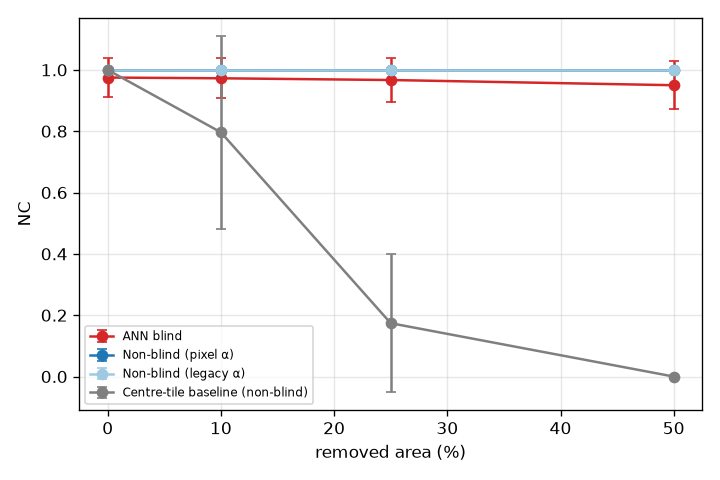
\includegraphics[width=\columnwidth]{cropping_curve.png}\caption{Crop response from the final held-out evaluation. Extraction paths have different reference information.}\label{fig:crop}\end{figure}

\subsection{Signal attacks and averaging}
As Table~\ref{tab:nc} shows, blind NC falls below .5 under JPEG quality 70 (.495) and quality 50 (.344), with BER .2433 and .3101. Gaussian noise produces NC .632. Blur produces NC .718, exceeding the host-assisted pixel-residual NC .392: filtering the marked image but subtracting an unfiltered host leaves a host-edge residual that can dominate the weak watermark. This is a property of that extractor under the specified attack, not a general proof that blind detection is superior.

Collusion averages independently watermarked copies of the same host, with the candidate's contribution attenuated as coalition size increases. Blind NC declines from .523 at $N=2$ to .188 at $N=100$; BER increases from .2318 to .3768. At threshold .125, blind CoRI is 1.00, .99, .81, .64, .60, and .60 across the six coalition sizes; its arithmetic aggregate is .774. The informed pixel extractor's corresponding aggregate is .801. Positive mean NC or a detection threshold crossing does not imply faithful bit reconstruction: the $N=100$ BER remains 37.68\%.

\begin{figure}[t]\centering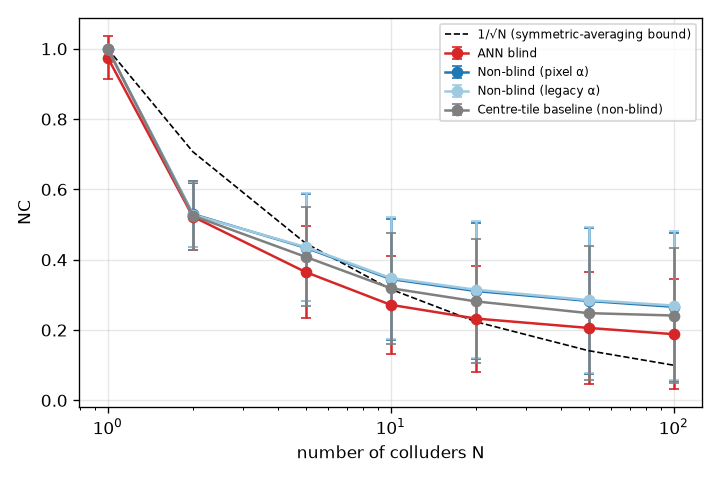
\includegraphics[width=\columnwidth]{collusion_curve.png}\caption{Candidate-watermark correlation versus averaged copy count in the final evaluation.}\label{fig:collusion}\end{figure}

The stored random-severity, mixed-attack ANN test set is a distinct protocol: across 360 test samples its NC is .6189 and BER is .1525. It should not be equated with the fixed-condition clean NC in Table~\ref{tab:nc}. On 120 unmarked held-out hosts the blind predictor has mean NC .0026 with standard deviation .0302 against assigned references and zero detections at .125. More stringent unrelated i.i.d. payload controls also show zero empirical false positives, while structurally similar generated text watermark controls exhibit substantially higher false-positive rates (.3583 in one mixed-ID control). Thus the idealized threshold is insufficient to guarantee low false alarms for every payload family.

\section{Discussion and Limitations}
Tiling improves crop recovery by preserving multiple intact or partly intact copies, and learned confidence pooling reduces reliance on damaged regions. The design does not establish a causal benefit uniquely attributable to the Catalan permutation: an isolated permutation ablation and comparison with other keyed mappings would be needed. The center baseline also differs in spatial support, embedding strength, and extractor information, so it is a demonstration of localization vulnerability rather than a controlled state-of-the-art comparison.

The low-amplitude spatial signal is vulnerable to quantization and low-pass processing; stronger or lower-frequency embedding could improve JPEG resistance at a visibility cost. Grid-based folding is sensitive to rotation, scaling, translations, and crop-and-resize misalignment, none of which are validated here. The receiver requires the correct key; keyed scrambling is not an authentication or cryptographic security guarantee. A colluder average is symmetric and diminishes any one independent mark. Strong tracing of large coalitions would require a suitable fingerprint code, longer payload, or additional side information. Finally, host and payload splits are isolated within DIV2K, but cross-dataset performance remains untested.

\section{Conclusion}
The completed hybrid framework combines keyed payload permutation, 64-fold mosaic placement, adaptive YIQ embedding, and a trained host-free extractor. Its final held-out results demonstrate high clean-image quality and strong recovery under tested aligned cropping, including 50\% area removal. JPEG compression and increasing coalition size markedly reduce recovered correlation and bit accuracy. Future experiments should isolate each component through ablations, test geometric synchronization and external hosts, calibrate false alarms for the actual payload distribution, and investigate frequency-domain embedding and coded fingerprinting.

\begin{thebibliography}{00}
\bibitem{wang2004ssim} Z. Wang, A. C. Bovik, H. R. Sheikh, and E. P. Simoncelli, ``Image quality assessment: From error visibility to structural similarity,'' \emph{IEEE Trans. Image Process.}, vol. 13, no. 4, pp. 600--612, 2004.
\bibitem{zhu2018hidden} J. Zhu, R. Kaplan, J. Johnson, and L. Fei-Fei, ``HiDDeN: Hiding data with deep networks,'' in \emph{Proc. ECCV}, 2018, pp. 657--672.
\bibitem{ahmadi2020redmark} M. Ahmadi, A. Norouzi, N. Karimi, S. Samavi, and A. Emami, ``ReDMark: Framework for residual diffusion watermarking based on deep networks,'' \emph{Expert Syst. Appl.}, vol. 146, 2020, Art. no. 113157.
\bibitem{agustsson2017ntire} E. Agustsson and R. Timofte, ``NTIRE 2017 challenge on single image super-resolution: Dataset and study,'' in \emph{Proc. CVPR Workshops}, 2017, pp. 126--135.
\bibitem{boneh1998collusion} D. Boneh and J. Shaw, ``Collusion-secure fingerprinting for digital data,'' \emph{IEEE Trans. Inf. Theory}, vol. 44, no. 5, pp. 1897--1905, 1998.
\bibitem{tardos2008optimal} G. Tardos, ``Optimal probabilistic fingerprint codes,'' \emph{J. ACM}, vol. 55, no. 2, Art. no. 10, 2008.
\end{thebibliography}
\end{document}
